\documentclass[margin=5mm]{standalone}
\usepackage{tikz}
\usepackage{array}
\usetikzlibrary{positioning, arrows.meta, calc, shapes.geometric}

\begin{document}
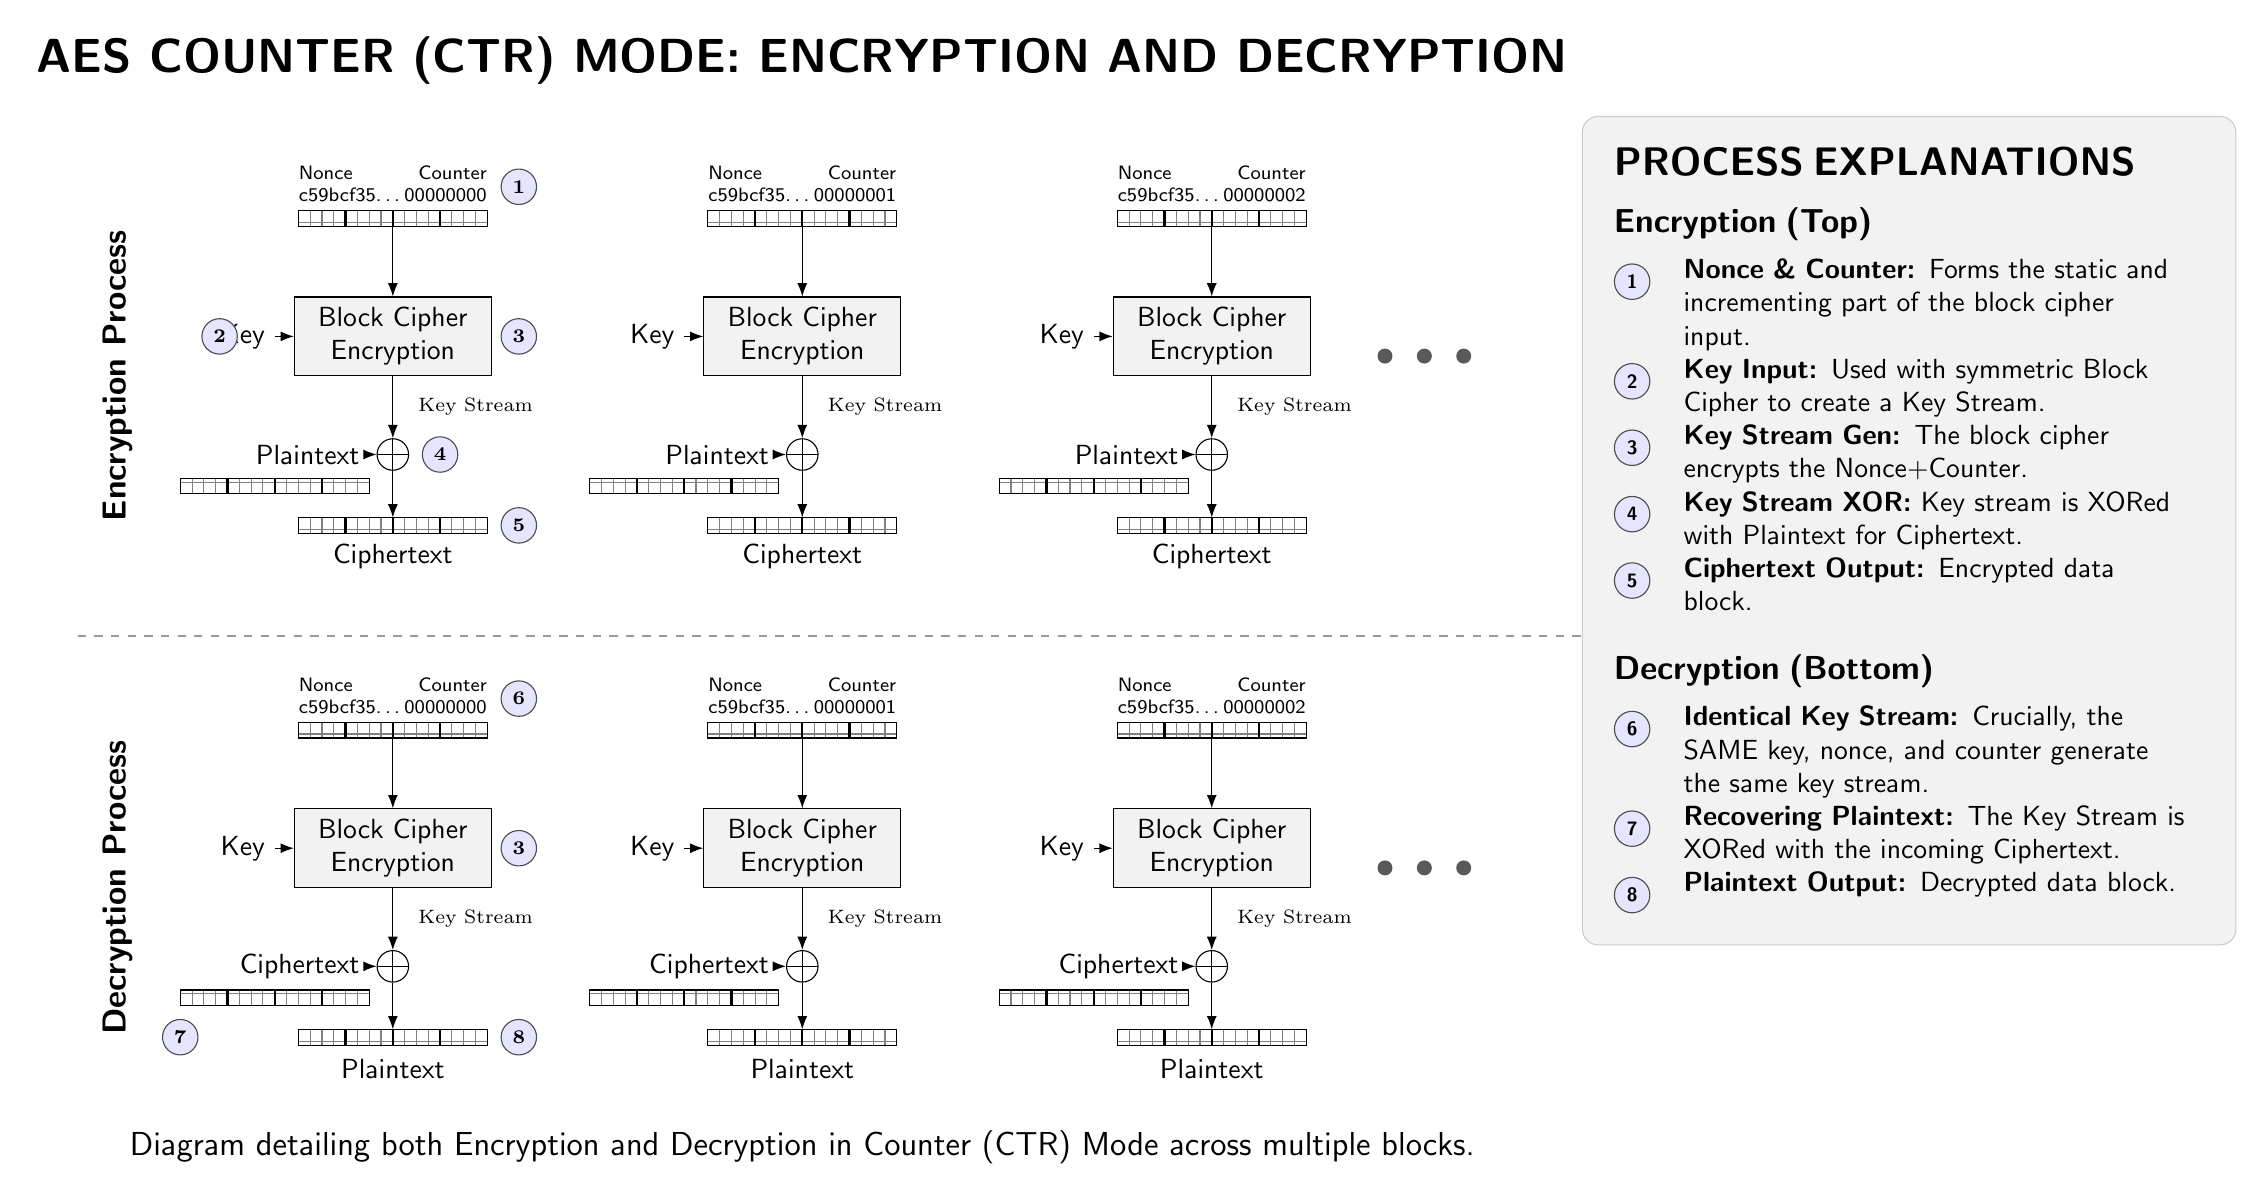
\begin{tikzpicture}[
    >=Latex,
    font=\sffamily,
    cipher/.style={draw, minimum width=2.5cm, minimum height=1cm, align=center, fill=black!5},
    xor/.style={draw, circle, inner sep=0pt, minimum size=0.4cm, path picture={
        \draw (path picture bounding box.north) -- (path picture bounding box.south) 
              (path picture bounding box.east) -- (path picture bounding box.west);
    }},
    indicator/.style={circle, draw=black!70, fill=blue!10, inner sep=0pt, minimum size=4.5mm, font=\scriptsize\bfseries, align=center},
    section title/.style={font=\Large\bfseries\sffamily, anchor=west}
]

% Set horizontal distance between blocks
\def\xstep{5.2}
% Set vertical offset for the decryption section
\def\yoffset{-6.5}

% Titles
\node[font=\LARGE\bfseries\sffamily, anchor=center] at (\xstep, 5.5) {AES COUNTER (CTR) MODE: ENCRYPTION AND DECRYPTION};
\node[rotate=90, font=\large\bfseries\sffamily] at (-3.5, 1.5) {Encryption Process};
\node[rotate=90, font=\large\bfseries\sffamily] at (-3.5, \yoffset + 1.5) {Decryption Process};

% --- LOOP FOR ENCRYPTION AND DECRYPTION BLOCKS ---
\foreach \i/\ctr in {0/00000000, 1/00000001, 2/00000002} {
    \begin{scope}[xshift=\i*\xstep cm]
        
        % ==========================================
        % ENCRYPTION PROCESS (TOP)
        % ==========================================
        
        % Nonce and Counter Labels
        \node[align=left, anchor=south west, inner sep=0, font=\scriptsize\sffamily] at (-1.2, 3.7) {Nonce\\c59bcf35\dots};
        \node[align=right, anchor=south east, inner sep=0, font=\scriptsize\sffamily] (counterTop) at (1.2, 3.7) {Counter\\\ctr};

        % Indicator 1 (Only on first block)
        \ifnum\i=0 \node[indicator] at (1.6, 3.9) {1}; \fi

        % Input register grid
        \draw[gray, thin, step=0.15cm, fill=gray!20] (-1.2, 3.4) grid (1.2, 3.6);
        \draw (-1.2, 3.4) rectangle (1.2, 3.6);
        \draw[thick] (-0.6, 3.4) -- (-0.6, 3.6) (0, 3.4) -- (0, 3.6) (0.6, 3.4) -- (0.6, 3.6);

        % Block Cipher
        \node[cipher] (encTop) at (0, 2) {Block Cipher\\Encryption};
        \draw[->] (0, 3.4) -- (encTop);

        % Indicator 3
        \ifnum\i=0 \node[indicator] at (1.6, 2) {3}; \fi

        % Key input
        \node[anchor=east] (keyTop) at (-1.5, 2) {Key};
        \draw[->] (keyTop) -- (encTop);
        \ifnum\i=0 \node[indicator] at (-2.2, 2) {2}; \fi

        % XOR operator and Key Stream Label
        \node[xor] (xorTop) at (0, 0.5) {};
        \draw[->] (encTop) -- (xorTop) node[midway, right, xshift=2mm, font=\scriptsize] {Key Stream};
        \ifnum\i=0 \node[indicator] at (0.6, 0.5) {4}; \fi

        % Plaintext Label & Arrow
        \node[anchor=east] (ptTop) at (-0.3, 0.5) {Plaintext};
        \draw[->] (ptTop) -- (xorTop);
        
        % Plaintext register grid
        \draw[gray, thin, step=0.15cm] (-2.7, 0.0) grid (-0.3, 0.2);
        \draw (-2.7, 0.0) rectangle (-0.3, 0.2);
        \draw[thick] (-2.1, 0.0) -- (-2.1, 0.2) (-1.5, 0.0) -- (-1.5, 0.2) (-0.9, 0.0) -- (-0.9, 0.2);

        % Ciphertext register grid & Label
        \draw[gray, thin, step=0.15cm, fill=gray!40] (-1.2, -0.5) grid (1.2, -0.3);
        \draw (-1.2, -0.5) rectangle (1.2, -0.3);
        \draw[thick] (-0.6, -0.5) -- (-0.6, -0.3) (0, -0.5) -- (0, -0.3) (0.6, -0.5) -- (0.6, -0.3);
        \node at (0, -0.8) {Ciphertext};
        \draw[->] (xorTop) -- (0, -0.3);
        \ifnum\i=0 \node[indicator] at (1.6, -0.4) {5}; \fi

        % ==========================================
        % DECRYPTION PROCESS (BOTTOM)
        % ==========================================
        \begin{scope}[yshift=\yoffset cm]
            
            % Nonce and Counter Labels
            \node[align=left, anchor=south west, inner sep=0, font=\scriptsize\sffamily] at (-1.2, 3.7) {Nonce\\c59bcf35\dots};
            \node[align=right, anchor=south east, inner sep=0, font=\scriptsize\sffamily] at (1.2, 3.7) {Counter\\\ctr};
            \ifnum\i=0 \node[indicator] at (1.6, 3.9) {6}; \fi

            % Input register grid (Same as top)
            \draw[gray, thin, step=0.15cm, fill=cyan!10] (-1.2, 3.4) grid (1.2, 3.6);
            \draw (-1.2, 3.4) rectangle (1.2, 3.6);
            \draw[thick] (-0.6, 3.4) -- (-0.6, 3.6) (0, 3.4) -- (0, 3.6) (0.6, 3.4) -- (0.6, 3.6);

            % Block Cipher (Still ENCRYPTION!)
            \node[cipher] (encBot) at (0, 2) {Block Cipher\\Encryption};
            \draw[->] (0, 3.4) -- (encBot);
            \ifnum\i=0 \node[indicator] at (1.6, 2) {3}; \fi

            % Key input
            \node[anchor=east] (keyBot) at (-1.5, 2) {Key};
            \draw[->] (keyBot) -- (encBot);

            % XOR operator
            \node[xor] (xorBot) at (0, 0.5) {};
            \draw[->] (encBot) -- (xorBot) node[midway, right, xshift=2mm, font=\scriptsize] {Key Stream};

            % Ciphertext Input Label & Arrow (Bottom)
            \node[anchor=east] (ctBot) at (-0.3, 0.5) {Ciphertext};
            \draw[->] (ctBot) -- (xorBot);
            
            % Ciphertext register grid (Input to XOR)
            \draw[gray, thin, step=0.15cm, fill=gray!40] (-2.7, 0.0) grid (-0.3, 0.2);
            \draw (-2.7, 0.0) rectangle (-0.3, 0.2);
            \draw[thick] (-2.1, 0.0) -- (-2.1, 0.2) (-1.5, 0.0) -- (-1.5, 0.2) (-0.9, 0.0) -- (-0.9, 0.2);
            \ifnum\i=0 \node[indicator] at (-2.7, -0.4) {7}; \fi

            % Plaintext Output register grid & Label
            \draw[gray, thin, step=0.15cm] (-1.2, -0.5) grid (1.2, -0.3);
            \draw (-1.2, -0.5) rectangle (1.2, -0.3);
            \draw[thick] (-0.6, -0.5) -- (-0.6, -0.3) (0, -0.5) -- (0, -0.3) (0.6, -0.5) -- (0.6, -0.3);
            \node at (0, -0.8) {Plaintext};
            \draw[->] (xorBot) -- (0, -0.3);
            \ifnum\i=0 \node[indicator] at (1.6, -0.4) {8}; \fi

        \end{scope}
    \end{scope}
}

% Continuation dots for both top and bottom
\begin{scope}[xshift=2*\xstep cm]
    \foreach \x in {2.2, 2.7, 3.2} {
        \filldraw[gray!70!black] (\x, 1.75) circle (2.5pt);
        \filldraw[gray!70!black] (\x, \yoffset + 1.75) circle (2.5pt);
    }
\end{scope}

% Dashed line separating Encryption and Decryption
\draw[dashed, thick, gray!80] (-4, -1.8) -- (3*\xstep, -1.8);

% ==========================================
% EXPLANATORY SIDE PANEL
% ==========================================
\node[anchor=north west, fill=black!5, draw=black!20, rounded corners=2mm, inner sep=4mm, text width=7.5cm, align=left] at (3*\xstep - 0.5, 4.8) {
    \textbf{\Large PROCESS EXPLANATIONS}\\[3mm]
    
    \textbf{\large Encryption (Top)}\\[1.5mm]
    % Use a tabular environment to force perfect text wrapping and indentation
    \begin{tabular}{@{}c >{\raggedright\arraybackslash}p{6.4cm}@{}}
        \tikz[baseline=-0.8ex]{\node[indicator]{1};} & \textbf{Nonce \& Counter:} Forms the static and incrementing part of the block cipher input.\\[1.5mm]
        \tikz[baseline=-0.8ex]{\node[indicator]{2};} & \textbf{Key Input:} Used with symmetric Block Cipher to create a Key Stream.\\[1.5mm]
        \tikz[baseline=-0.8ex]{\node[indicator]{3};} & \textbf{Key Stream Gen:} The block cipher encrypts the Nonce+Counter.\\[1.5mm]
        \tikz[baseline=-0.8ex]{\node[indicator]{4};} & \textbf{Key Stream XOR:} Key stream is XORed with Plaintext for Ciphertext.\\[1.5mm]
        \tikz[baseline=-0.8ex]{\node[indicator]{5};} & \textbf{Ciphertext Output:} Encrypted data block.
    \end{tabular}\\[4mm]
    
    \textbf{\large Decryption (Bottom)}\\[1.5mm]
    \begin{tabular}{@{}c >{\raggedright\arraybackslash}p{6.4cm}@{}}
        \tikz[baseline=-0.8ex]{\node[indicator]{6};} & \textbf{Identical Key Stream:} Crucially, the SAME key, nonce, and counter generate the same key stream.\\[1.5mm]
        \tikz[baseline=-0.8ex]{\node[indicator]{7};} & \textbf{Recovering Plaintext:} The Key Stream is XORed with the incoming Ciphertext.\\[1.5mm]
        \tikz[baseline=-0.8ex]{\node[indicator]{8};} & \textbf{Plaintext Output:} Decrypted data block.
    \end{tabular}
};

% Bottom Caption
\node[font=\large\sffamily, anchor=center] at (\xstep, \yoffset - 1.8) {Diagram detailing both Encryption and Decryption in Counter (CTR) Mode across multiple blocks.};

\end{tikzpicture}
\end{document}
